% ssb-paper-2018/main.tex

\documentclass[9pt,sigconf]{acmart}
% \documentclass[sigconf]{acmart}
% \settopmatter{printfolios=true}

\usepackage{balance}


\title[Secure Scuttlebutt: An Identity-Centric Protocol
       for Subjective and Decentralized Applications]{%
  Secure Scuttlebutt: An Identity-Centric Protocol \\
  for Subjective and Decentralized Applications
}

% \tt\small ( \today\ / last commit was \input{.git/refs/heads/master})}

% \title{Replicated append-only logs as as basis for decentralized
% information-centric applications: An analysis of Secure Scuttlebutt}

\author{Dominic Tarr}
\affiliation{ssb:@EMovhfIrFk4NihAKnRNhrf}
\email{RaqIhBv1Wj8pTxJNgvCCY=.ed25519}

\author{Erick Lavoie}
\affiliation{McGill University, Montreal, Canada}
\email{erick.lavoie@mail.mcgill.ca}

\author{Aljoscha Meyer}
\affiliation{TU Berlin, Germany}
\email{aljoscha.t.meyer@campus.tu-berlin.de}

\author{Christian Tschudin}
\affiliation{University of Basel, Switzerland}
\email{christian.tschudin@unibas.ch}


\acmConference[ICN'19]{ACM ICN'19 conference}{Sep 24-26, 2019}{Macau, Macao}
\acmYear{2019}
\acmDOI{10.1145/1111111.9999999}
\acmISBN{978-1-4503-9999-9/19/09}
\copyrightyear{2019}
\setcopyright{rightsretained}

 \begin{CCSXML}
<ccs2012>
<concept>
<concept_id>10003033.10003034</concept_id>
<concept_desc>Networks~Network architectures</concept_desc>
<concept_significance>500</concept_significance>
</concept>
<concept>
<concept_id>10011007.10010940.10010971.10010972.10010975</concept_id>
<concept_desc>Software and its engineering~Publish-subscribe / event-based architectures</concept_desc>
<concept_significance>500</concept_significance>
</concept>
<concept>
<concept_id>10010520.10010521.10010537.10010540</concept_id>
<concept_desc>Computer systems organization~Peer-to-peer architectures</concept_desc>
<concept_significance>300</concept_significance>
</concept>
<concept>
<concept_id>10002951.10003152.10003161.10003162.10003414</concept_id>
<concept_desc>Information systems~Linked lists</concept_desc>
<concept_significance>300</concept_significance>
</concept>
</ccs2012>
\end{CCSXML}

\ccsdesc[300]{Networks~Network architectures}
\ccsdesc[300]{Software and its engineering~Publish-subscribe / event-based architectures}
\ccsdesc[300]{Computer systems organization~Peer-to-peer architectures}
\ccsdesc[300]{Information systems~Linked lists}

\keywords{Secure Scuttlebutt, Information-Centric Networking, Push vs.~Pull}

% ----------------------------------------------------------------------
\begin{document}

% TODO: clean up terminology (feed/log/author/identity/id, server/relay/device/node/peer/machine, message/data/entry, ``social graph'', subjectivity (subjective reader) as opposed to plurality (how to interpret messages))

\begin{abstract}
  Secure Scuttlebutt (SSB) is a novel peer-to-peer
  event-sharing protocol and architecture for social apps. In this
  paper we describe SSB's features, its operations as well as the
  rationale behind the design. We also provide a comparison with Named
  Data Networking (NDN), an existing information-centric networking
  architecture, to motivate a larger exploration of the design space
  for information-centric networking primitives by formulating an
  identity-centric approach. We finally discuss SSB's limitations
  and evolution opportunities.

%  At the transport level, SSB is a replication protocol for
%  append-only logs.  applications communicate indirectly by writing to
%  the local node's log and by reading from the locally available
%  replicated logs. From these, each app instance constructs its own
%  intepretation of the shared app state (an approach called
%  ``subjective reader'').  Scaling is achieved through in-network
%  caching of the immutable log updates and by routing the content
%  along the social graph.

%  SSB's current set of applications include classical social media
%  apps (chat, with end-to-end encryption and meta-data privacy), game
%  and lifestyle apps (chess, book reviews) as well as technical
%  applications like a p2p git, a shared file system, or a social
%  backup app for crypto keys using a secret sharing protocol.
\end{abstract}

\maketitle


% ----------------------------------------------------------------------
\section{Introduction}

A simple conceptual architecture for community applications consists
of a global data pool to which every person can contribute and where
every person can tap into the shared data~-- data sharing being the
purpose of such applications. This model still is valid if one adds
access control to the picture, either tied to the data (encryption
giving access to content only to entitled holders of the decryption
keys) or encrypting data in transit (login and TLS). Facebook and
other centrally organized social app service providers fit well under
this global data pool model but have been strongly criticized for
abusing their central provisioning position.  The ``decentralized web
movement''~\cite{decent-2018-aug} is the most visible technical
response to this critique, pointing out implementation alternatives.

One of these alternatives is a project called Secure Scuttlebutt (SSB)
that started in 2014. After several iterations of protocol design and
implementation, SSB has become a stable service for over 10,000 users
offering them rich media community applications with strong
cryptographic protection (end-to-end encryption and metadata privacy)
and running in pure peer-to-peer mode.

\subsection*{Selective Complete Log Replication}

SSB relies on the core insight that each  participant is only interested in a \textit{subset} of the global data pool, thus it is feasible to locally store all the data a participant is interested in. To partition the data pool, all data is associated with the \textit{identity} that produced it. Participants select their slice of the data pool by specifying the set of identities whose data they care about. This creates a ``social graph'' along whose edges data flows (Figure~\ref{fig:net-of-people}). Even as the overall system scales, the amount of data any single peer is interested in and thus needs to handle stays roughly the same.

Each participant can publish data to their single-writer, append-only log. This choice of data structure allows efficient replication and verification of the integrity of received data. Replicating these larger slices of the data pool comes with an unusual set of tradeoffs, discussed throughout the paper. As it turns out, replicated logs form a solid foundation for implementing many classes of applications.

% SSB's spin on the above conceptual model is that all participants {\em
%   replicate the global data pool}, which enables off-line operations,
% avoids redundant data transfers and has become feasible --~at least in
% principle~-- because storage nowadays is a cheap resource, just that
% the sheer volume of social app data prohibits a full
% replication. However, because a participant is mostly interested in
% content from its peers, which is a very small number compared to all
% participants, only portions of the global data pool need be
% replicated. This observation is leveraged in SSB's transport layer
% which is tasked to {\em selectively replicate} the global data pool
% {\em along the edges of the social graph}, as we will explain in
% Section~\ref{sect:XX}.

\begin{figure}[htb]
  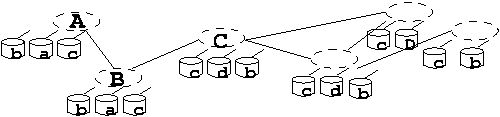
\includegraphics[width=0.9\columnwidth]{figs/net-of-people.pdf}
  \caption{SSB's ``Internet of Identities'' -- {\rm\small Users A, B and C
      replicate logs ({\em a, b, \ldots}) based on whom they follow: {\em C} does not follow {\em A}, hence has no log {\em a}. {\em A} and {\em B} follow each other such that when {\em A} follows {\em C}, {\em A} will get {\em C's} log {\em c} via {\em B:} new content is pushed directly if possible and through intermediary friends if necessary.
    }\label{fig:net-of-people}}
\end{figure}

% A second spin of SSB is that replication is done {\em pro-actively} and
% at the granularity of the {\em complete input by a single peer} to the
% global data pool. This novel way of implementing the global data pool
% model is in stark contrast to current solutions where central server
% repositories hosting this pool are accessed by client software in an
% on-demand fashion, assuming a storage-less end-device. Today's data
% dissemination mode is reactive (client-server protocol to fetch data)
% and piecemeal (only the instantly needed data items are requested,
% possibly multiple times, and bundled with fresh ads, as the client
% does not necessarily cache all requested data). In SSB however, the
% central objects are the {\em complete} collection of a specific peer's
% input to the pool, organized as an append-only log. In
% Sections~\ref{sect:XX} and~\ref{sect:XX} we will explain the
% advantages of this approach (trust, off-line operations and efficient
% real-time notifications), and discuss its drawbacks (index building,
% lack of delete operation, storage bloat, re-keying).

\subsection*{Subjective Reader}

Because replication in SSB is selective and driven by a peer's
social graph, different end devices will have access to different sets
of log replicas, leading to different views of the world, which we call
a ``subjective reader'' approach. SSB considers this a desirable
property: each peer is free to
consider data sources of its own choosing instead of having to feed
from a centrally provisioned or otherwise converged view. While it is
possible to implement consensus protocols over SSB, or to designate
central data aggregators from which many peers consume the
consolidated outputs, the SSB network itself deliberately doesn't
offer consensus services nor central content (directories etc). In
Section~\ref{ssect:dapps} we will show the implications of this
technological choice on the structure of distributed applications that
can only read from and write to local logs.

\subsection*{Novelty}

Putting complete replication of individual append-only logs at the
core of SSB's protocol avoids several hard problems in distributed
systems. {\bf First}, it is a radically decentralized approach
requiring only minimal specification-level coordination among the
participants but no run-time checks or configuration
management.
% Typically, active/active multi-master replication in
% databases, which comes closest to SSB's approach, requires tight
% configuration control while in SSB, existing peers can go offline and
% new peers can come and go at any time, at the price of weak
% consistency guarantees, though.
{\bf Second}, although append-only
data structures are well known for their benefits and are at the core
of crypto currencies' consensus finding, SSB uses logs without any
consensus properties. The issue is deliberately sidestepped, but all
necessary building blocks are provided to higher layers.
% Quite on the contrary, SSB completely sidesteps
% consensus but provides the building blocks for implementing it the hooks for implementing service abstractions
% like tangles for implementing CRDTs on top of SSB i.e., eventual
% consistency.
{\bf Third}, crafting a cryptographic ID system and
maintaining a social graph that informs routing creates a very narrow
filter: it implements a receiver-driven approach where
data only flows where it is needed and provides flexibility in the actual data dissemination strategy.
%without imposing any
%fine-grained request/reply protocol.
%%Instead, any dissemination
%technology is adequate, including broadcast and push mode, because
%network elements can verify data validity (due to the logs' signed
%entries) and monotonicity of the updates without additional key and
%certificate material, guaranteeing that only valid traffic is
%propagated at any forwarding step.
{\bf Fourth}, it makes every peer a
publisher by design. This property goes beyond the decentralized
approaches like DAT~\cite{datproject} or IPFS~\cite{benet2014ipfs} which assume that there
exist replication servers but keep the separation between a data
transport network and a server layer.
% In SSB, bidirectional
% communications is only possible if both parties {\em are}
% repositories.
{\bf Last but not least}, log replication leads to a
distributed system with inherent high resilience as any communicating
element carries a persistent copy of the data. In traditional distributed
systems, coordinating the data persistence as a basis for resilience
is often an add-on task, or requires at least a special recovery
service.

\subsection*{Comparing SSB to NDN}

Despite SSB data replication being currently implemented as an
application protocol (layer 7 in the OSI
stack~\cite{briscoe2000understanding}), we believe that its underlying
principles are worth studying from a network API perspective (layer 3 in
the OSI stack) to highlight regions of the design space that could be
further investigated. We sketch here some aspects in which SSB differs
from \textit{Named Data Networking} (NDN)~\cite{ahlgren2012survey}, a
popular proposal for Information-Centric Networking (ICN). A longer
exposition of SSB's underlying communication model is available in a
separate publication~\cite{tschudin2019broadcast}.

In SSB, the delivery of information is organized around \textit{named
  data streams} for signed events. The basic unit of addressing is a
full log that might still produce new event messages in the future.
The SSB streams guarantee \textit{reliable causal
  ordering}~\cite{cachin2011introduction} and \textit{authenticity}.

Delivery of streams follows a \textit{push model}: once a receiver has expressed interest in a stream, new items are transferred automatically without being requested individually. Flow-control (back-pressure) in the current overlay implementation is done implicitly by the TCP connections used to deliver data among peers.

Streams are tied to a single \textit{identity} with a corresponding
\textit{public key}\/: only this identity can produce new items in the
stream with the correct signature.  Because the signature ensures the
integrity of the items, they can be served from anywhere and by
anybody.
% Erick: The identity producing the stream may therefore be mobile.
% cft: ``therefore'' is not true: ``serving by anybody'' is not related to mobility.
Moreover, users independently create the key that serves as an
identity. Streams are therefore
\textit{self-certifying}~\cite{mazieres1998selfcertifyingpathnames}
and their integrity does not rely on an external trust anchor nor a
central naming authority or other name coordination and allocation
mechanisms.

In contrast, NDN embodies quite different design choices. First, the basic elements of networking are \textit{single pieces of data}, identified by hierarchical names similar to paths in a filesystem. Second, data is accessed via a \textit{pull} model: a consumer issues an \textit{interest} in a name, and the network delivers the corresponding data. Third, many NDN schemes rely on a hierarchical trust model to issue certificates that can in turn be used to sign individual pieces of data.\footnote{See~\cite{zhu2012chronos} for a proposal that leverages a web of trust model in a decentralized chat application built on top of NDN.}

%%A core contribution of this paper is a direct comparison of SSB with
%%\textit{named data networking} (NDN). Our analysis reveals strong incompatibilities in at least two
%dimensions. The first is the content dissemination strategy where NDN
%is well known for its PULL pattern while SSB follows a PUSH model.
%\vskip 0.5em
%
%\begin{tabular}{l|c|c|}
%                   &     PULL                  & PUSH \\
%\hline
%  name-centric     & {\bf NDN}     & {\small\em NDN-over-SSB?} \\
%                   &               & {\small\em Sect.~\ref{ssect:ndn-over-ssb}} \\
%\hline
%  identity-centric & {\small\em SSB-over-NDN?} & {\bf SSB}               \\
%                   & {\small\em Sect.~\ref{ssect:ssb-over-ndn}} & \\
%\hline
%\end{tabular}
%\vskip 0.5em
%
%The second difference is more subtle and seems to be rooted in what
%NDN considers the main focus of networking. In NDN,
%repositories are an implicit assumption on which the scalability
%claims of NDN rest, and consequently, these repositories --- or, to be
%more precise, their global prefixes and all names attached to them ---
%are points of centralization. SSB, on the other hand, has no global
%constructs, true to its decentralized point of view, and can be called
%{\em identity-centric} in order to contrast it from {\em name-centric}
%NDN.

It is not clear that either design can subsume the other: one can implement SSB over NDN or the opposite but each option comes with significant runtime costs. Still, there could be an intermediate territory where a future synthesis of the two approaches may emerge. We therefore analyze the trade-offs that appear in various ways of layering NDN and SSB to enrich the discussion around future developments in ICN.

%Then, after a brief introduction to NDN on a similar conceptual level, we examine how these models can emulate each other. We then use these lessons to sketch a fruitful way of combining SSB with NDN.

%, but we have not
%progress so far in our analysis, yet.


% \subsection*{Scuttlebutt = Information-Centric Gossip}
%
% \ldots\ why this name
% \ldots\ it applies to the app-level, and can apply to the network layer, but doesn't have to: any dissemination method works for gossip.
% \ldots\ some words about the SSB community, available documentation, past evolution, subjective roadmap \cite{ssb-consortium, tarr:ssb-notes,ssb-on-web,ssb-protocol-guide-2018,staltz-roadmap-2019}

\subsection*{Structure of this paper}

We start out by giving an overview of the SSB protocol in Section \ref{sect:architecture}. Next we describe common patterns of how applications can be built on SSB (Section \ref{sect:apps}). We show how SSB relates to other networking protocols, first through a detailed comparison with NDN (Section \ref{sect:NDN}) and then in the broader context of related work (Section \ref{sect:relwork}). We conclude the paper with an outlook on some of the ``work in progress'' (Section \ref{sec:wip}) and an evaluation of the problems (Section \ref{sect:nay}) and benefits (Section \ref{sect:yay}) of the SSB approach.


% ----------------------------------------------------------------------
\section{SSB Architecture and Protocol}
\label{sect:architecture}

In SSB, each user is identified by an ed25519~\cite{bernstein2012high} keypair. Since anybody can generate a random keypair with very low probability of multiple peers generating the same keypair, no central authority is necessary for introducing users to the system. Conceptually, SSB is a network of identities that connect to each other (physical topology) and share mutual or unilateral interest in the other peer's data (social graph), as shown in Figure~\ref{fig:net-of-people}. A node running the SSB protocol is called a \textit{relay}. The identity that holds the private key of a log is called its \textit{author}.

The {\em single-writer append-only logs} of SSB consist of entries (called \textit{messages}) that include a {\em backlink} in the form of a cryptographic hash of the previous message (or a special indicator for the first message of a log). The most distinguishing feature of this linked list, when compared to a regular blockchain, is that each SSB user maintains their own log and cryptographically signs all their (and only their) messages. Messages whose backlink points to a message in a different log (i.e. by a different author) are considered invalid and will be rejected by SSB relays.

These constraints still allow creation of arbitrary trees rather than logs. To enforce log structure, each SSB relay checks that every message has exactly zero or one incoming backlinks. If it has more than one, the log is considered {\em forked}. All messages from the point of the fork onwards are ignored, the log cannot be appended to anymore.

Concretely, each message, which may not exceed 4 KB, contains the following pieces of data~\cite{ssb-spec-messages}:

\begin{itemize}

\item the {\em backlink} to the previous message, or a null value

\item the public key of the message's {\em author}

\item the {\em sequence number} of the message, which must be one more than the sequence number of the previous message, or exactly one if it is the first message of the log

\item a claimed {\em timestamp} of when the message was created

\item a {\em hash} indicator that specifies the concrete hash function that was used to compute the backlink

\item the {\em content} of the message

\item the author's {\em signature} over all the previous data

\end{itemize}

In the current version of SSB, {\em content} is a JSON object that must contain a {\em type} key that serves as a hint for how the content should be interpreted. SSB enforces that the content is valid JSON by rejecting any malformed message.
Encrypted content is represented as a base64-encoded string, together with a tag that signifies which encryption algorithm was used.

SSB defines a format for encoding specifically the public keys of identities and the hashes of messages and blobs (see below) as strings. This allows applications to scan the content of messages from other authors for such references, e.g. in order to create database indices (see Sect.~\ref{ssect:dapps}).

% The precise, byte-for-byte definition of the json-based message encoding is given in \cite{ssb-spec-messages}.

\subsection*{Replication}

The principal function of SSB relays is to connect to other relays and exchange log {\em updates}. To do so, relays maintain a point-to-point encrypted~\cite{tarr2015secrethandshake} overlay network over which they run a gossip protocol. When two relays start gossiping, they exchange the current sequence numbers of all logs they are interested in. If a relay receives a lower sequence number for a log than it sent, it transmits the messages that the other relay is lacking. If at a later point a new message of the log becomes available to a relay, it is automatically \textit{pushed} to the connected relays. As an optimization, this {\em eager} gossip is only performed over the edges of a spanning tree, which itself is maintained via the plumtree~\cite{leitao2007epidemic} protocol. In classic peer-to-peer fashion, clients (leaf nodes) are no different than relays except that they usually include some graphical user interface and perform application logic.

In addition to this primary replication mechanism, SSB provides two other ways of exchanging information. {\em Blobs} are content-addressed pieces of free-form data, typically images or other documents larger than the 4KB limit, that are referenced from messages but are not part of any log. They are not widely disseminated automatically, but rather fetched on demand via a simple request-flooding protocol. {\em Out-of-order messages} are a similar mechanism to address and fetch messages on demand via their hashes.

\subsection*{SSB Relays as an Application Platform}

Beyond replicating logs and checking the validity of update messages, an SSB relay offers an API to its peers. Peers can host arbitrary programs that issue remote procedure calls (RPCs) to the relay. The exposed functionality includes appending to a log (if you know its private key), reading from logs, requesting which logs a relay should replicate, and fetching blobs and out-of-order messages.
% SSB thus becomes a platform for building applications, encapsulating the complexity of data replication.

The reference implementation of the SSB relay~\cite{ssb-server}, written in JavaScript, also includes a mechanism for loading {\em plugins} into the relay to extend its functionality. There are a few default plugins: conceptually these can be thought of as client programs that are always running. Of particular importance are those that guide the replication process. The {\em friends} plugin~\cite{ssb-friends} scans the relay's log for specific messages that indicate which other identities the author {\em follows}. The plugin then instructs the relay to fetch and replicate these logs. These other logs might of course also contain some of these messages. The friends plugin transitively replicates these friends-of-a-friend logs as well, up to a configurable maximum distance in the friends graph.

Beyond ``befriending'' other authors through {\tt follow} messages (i.e. messages of type {\tt follow}), an SSB user can control the shape of their social graph via special {\tt block} messages which limit the transitive log replication. Both the {\tt follow} as well as {\tt block} messages are overheard by relays, through scanning all received log updates, and inform them about where updates should be delivered (or not). Decisions about whom to replicate can be --and in the current system is-- guided by the content of the very data that is replicated. By storing the relevant information inside the author's log (as opposed to a local or central database), other peers can use this informtion to guide their decisions.

The overlay network also makes use of logs to store configuration information, in this case the SSB\_ID-to-IP\_address mapping: operators publish the static IP addresses of highly-available relays (called {\em pubs}) to their log. When an SSB relay needs to connect to the overlay, the responsible plugin can scan any locally available log replica for this information.

\subsection*{SSB's Layered Architecture}

It is worth noticing that SSB spans three independent layers of protocols. The most fundamental protocol is the message format: all peers need to agree on what constitutes identities, valid messages, and how to compute hashes to address messages and blobs. This is the ``thin waist'' of SSB (see figure~\ref{fig:waist}).

\begin{figure}[htb]
  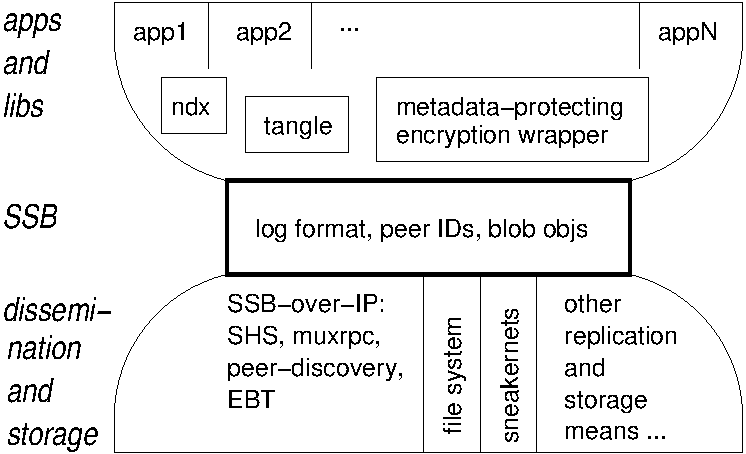
\includegraphics[width=0.9\columnwidth]{figs/ssb-waist.pdf}
  \caption{Secure Scuttlebutt's protocol stack.}
  \label{fig:waist}
\end{figure}

Next (below) is the specific mechanism by which relays exchange data. The default RPC mechanism is one option, but alternative mechanisms such as distribution via a sneakernet could also be used. Different peers that do not share a common replication mechanism could still interact indirectly, as long as there are some relays that understand multiple replication protocols.

In other words, the core logical replication protocol by which a relay serves its clients is fully independent from the actual dissemination protocols. And finally, the publishing and interpretation of application data in such messages is again a separate affair that is layered on top of the thin waist.

% ----------------------------------------------------------------------
\section{Distributed Apps and Data Structures over SSB}
\label{sect:apps}

% TODO: Rework to reflect the actual structure of the section
% TODO: Make title capitalization uniform

The replication model of SSB enables many collaborative applications to be implemented easily by abstracting much of the complexity in distributing the updates. However, implementing such applications still comes with challenges. To introduce them, we first discuss in detail the implementation of a user directory to introduce the implementation approach, then briefly cover other applications currently in use, and finally discuss some core issues that are shared between all applications.

\subsection{Example: SSB's user directory}
\label{ssect:about}

`{\small\tt about}' is SSB's user database i.e., an application that
associates cryptographic IDs with (typically) human-readable
attributes. A single message format has been defined to this end:
{\small\begin{verbatim}
'content': {
  'type'  : 'about',
  'about' : about_id,
  attr_name : attr_value   // multiple times
}
\end{verbatim}}

\noindent
The {\small\tt about} app scans all logs for messages of type {\small\tt
  `about'} and constructs a database as shown in
Figure~\ref{fig:about}, retaining the most recent attribute assignment
found. In this database, an {\small\tt about\_id} is associated with a list of key/value pairs which are prepended by the publishing author's ID. It is left to the end user's {\small\tt `about'} application to subjectively select which of these bindings should be displayed.
%To each target user ID we associate a directory where
%key/value pairs are collected on a per author basis (which is extracted
%from the message's envelope).
%
Currently the {\small\tt name}, textual {\small\tt description} and {\small\tt
  image} attributes are understood by most SSB user interfaces and are
used to substitute or decorate the cryptographic ID. If {\small\tt
  about\_id} and {\small\tt author\_id} are identical, this means that an
attribute was self-chosen and then is usually rendered with a higher preference
over key/value pairs assigned by others.

\begin{figure}[htb]
  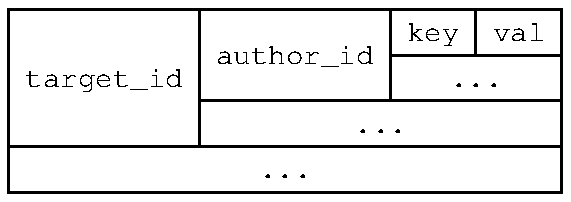
\includegraphics[width=0.6\columnwidth]{figs/about-ds.pdf}
  \caption{SSB's user directory data structure (after extraction from the logs).}
  \label{fig:about}
\end{figure}

\noindent
In terms of CRUD\footnote{Create, Read, Update, Delete} actions, creation happens once a new SSB identity adds
its own {\small\tt about} message to its log; reading the user database
is performed on the above data structure; updates are expressed by
adding an {\small\tt about} message --regardless whether it relates to
the author itself or to another identity-- to one's own (!) log and all peers
updating their extracted database; deleting a user entry is not
possible, at least not directly (one would have to block that user ID
as well as all IDs which wrote an update for that user).

There can never be confusion about the sequence or scope of attribute
assignments because they are orderd by the log (and thus in time) and
kept separate, per author ID. Note also the presence of the
``subjective reader'' property: the content of a peer's user database
is dependent on their position in the social graph. The ``subjective''
mindset is also visible by letting every user assign attributes to
anybody, leaving it to the user interface (and human viewer) to select
which of the self-chosen or given display names and images is most suitable
for a given ID.

\subsection{Profiles of other selected SSB apps}
\label{Section:AppProfiles}

Multiple applications have been written by contributors and are used daily by
the SSB community. The following selected examples represent
alternatives to well-known services and they illustrate both opportunities and
challenges of communication through replicated append-only logs.

\textit{Git-ssb}~\cite{git-ssb} is an alternative to GitHub~\cite{github} that
replicates git-based version-controlled code repositories through contributors
logs. It provides an encoding of repositories in SSB logs, a bridge to
interoperate with git repositories, and a web-based viewer to browse
repositories. The object model of Git~\cite{chacon2014pro} has a similar
structure to SSB's logs. Other git operations, such as creating repository, are
all SSB messages. Since any user can independently update the \textit{same} repository, as defined by its creation message, consensus on the "official" master branch and its latest commit is enforced
through social coordination. In case of concurrent updates to the same branch
in the same repository~\cite{git-ssb-push-conflict}, referencing both concurrent
updates in a later merge commit in effect resolves
the ambiguity.

\textit{Ssb-chess}~\cite{ssb-chess} is a correspondence chess application in
which players can invite one another to play, alternatively share their next
move until the game ends, and external observers can comment on the game.
Because the rules of chess preclude concurrency,  i.e. at any time there is always
 only one of the two participants that is permitted to modify the state of the chess board,
 a game can easily be represented as a linked list with nodes
representing chess moves alternating between the two participants' logs.
Moreover only the participants, explicitly mentioned in the original invitation, are
allowed to modify the state of the game. The implementation does not require
concurrency management and is therefore conceptually straight-forward.

\textit{Gatherings}~\cite{patch-gatherings} are alternatives to
Meetup~\cite{meetup.com} that enables participants to signal their intention to
attend or not attend to physical events. A gathering is defined by its creation message
but otherwise has no fixed properties. Anyone that has a reference to the creation message may
change its properties, such as location, start and end dates, description, and
image, by publishing an update message. The value of those properties are the
most recent set by anyone. Initially, recency was determined by the time of
creation, as reported by the user's client implementation (\textit{self-stated
creation time}). To be more robust to potential invalid
timestamps however, some client implementations have started using the time at
which message updates are \textit{received}, then disambiguate using the
self-stated creation time.

% \textit{Scuttle-poll}~\cite{scuttle-poll} is an implementation of the polling
% model of Loomio~\cite{loomio}, an online group decision-making platform. In
% addition, it serves as the basis for \textit{Scry}~\cite{patchbay-scry}, an
% alternative to Doodle~\cite{doodle.com}, itself an online calendar tool for
% organizing meeting. A poll is a request for opinions, which for example may
% express preference for one choice among many possibilities or provide a list of
% time availabilities. A poll is created by publishing a \texttt{poll} message in
% a log with a number of possible options and a deadline. Participants then
% publish their \textit{position} among the choices available. The poll creator
% finally publishes a \textit{resolution} based on the other participants'
% positions. Concurrency in polls is limited because the creation and resolution
% of the poll are done by the same user, and therefore works quite well with the
% SSB communication model.

%The fact that a small community with a dozen or so of core developers, which are self-funded
%and working mostly voluntarily, could produce alternative applications that
%work well enough to be used daily suggests the SSB communication model does
%make the implementation of common social applications (relatively) simple.

\subsection{Running Distributed Applications over Replicated Logs}
\label{ssect:dapps}

``Infrastructure-less'' distributed application as presented above
become possible because central servers can be fully replaced by each
peer working on its local set of replicated logs. In this subsection
we discuss the particularity of this approach and its constraints.

A common pattern of SSB's applications is that they heavily rely
on local database support for organizing the data contained in the logs.
Typically a map-reduce strategy is used where the map phase filters
the logs and the reduce actions computes the latest application state.

In the user directory application (Sect.~\ref{ssect:about}), the filtering is
done by selecting only {\tt about} messages for a specific target ID
and the reduce action consists in accumulating the latest key-value
pairs such that a more recent key-value pair replaces an older one if
it was signed by the same author\_id. The size of the replicated logs,
although locally stored, would lead to very long response times if the
map-reduce would be executed at render-time. Instead, almost each
application will build indexes and aggressively cache state that was
already aggregated. Should the indexes ever become corrupted
(e.g. because the user interface app crashed in the middle of a
complex indexing step), they can be fully regenerated from scratch.

An important aspect is whether the reduction step can be done in an
incremental fashion by reusing previously computed application state.
For example, counting the ``likes'' that a post receives works fine:
incoming log extensions are indexed and if they are of the like type,
the counter corresponding to the referenced message is incremented.

Other applications, however, may need a {\em full} re-evalution of the
reduce function each time the underlying index changes. An example for
this case is a chat in form of sequence of post messages: if some identity is added to
the set of followed identities, its log is incrementally replicated, and
so are the posts of this identity. For each incoming new post, which may
have been written very long ago, one has to insert it at the right
place. This problem is shown in Figure~\ref{fig:tangle} where a message
has not yet been replicated to a client and, once it arrives,
has to be properly inserted into the application-level data structure.

\begin{figure}[htb]
  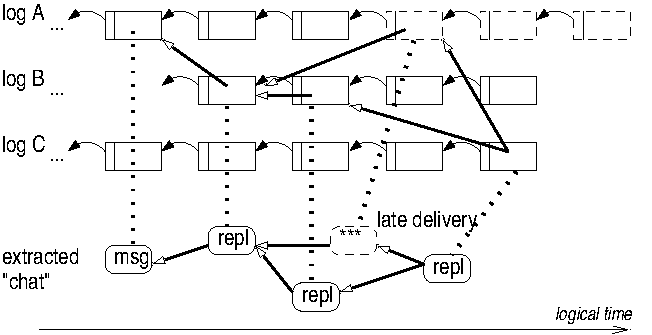
\includegraphics[width=0.9\columnwidth]{figs/tangle.pdf}
  \caption{Example of extracting application data spread over multiple collaborating logs and dealing
    with not-yet-delivered data.\label{fig:tangle}}
\end{figure}

A simple solution (adopted in some SSB client software) is to use the
timestamp claimed by the author of the post, and in this case one can
reuse the existing time-sorted list and insert the new post. However,
because an author could lie about the timestamp, the reduce function
should do a topological sort  based on the causality relationship with
other posts and their replies, which form a directed acyclic graph.
\footnote{Writers can facilitate the causal ordering by explicitly referring to the most recent messages in other logs they were aware of at the time of writing, regardless of whether the content was directly relevant to their own message. We call the graphs resulting from this pattern "tangles".} Insertion into the dependency graph may or may not lead to having to rerun the sort on the whole graph of
postings. Clearly, the lack of a central server hosting the reference
list of posts and being able to record a post's submission time, leads
to more complex client software that must prepare for and defend
against a broad range of adversarial data found in the logs.

%Storing this transitive closure of application-level graphs in a space-efficient way such that it can be quickly queried and efficiently updated is a difficult but well-studied problem in the database literature~\cite{jin2012scarab,yildirim2013dagger}. It should be possible to leverage some properties of SSB to get higher-quality results. The immutability of messages reduces the number of cases when dynamically maintaining the index structure, and the fact that each feed forms a total order can be utilized to efficiently encode the relation. Designing and implementing a general framework for performing causal ordering queries on SSB messages would be both an interesting research topic and a powerful tool for building applications

\subsection{Synchronization and Eventual Consistency}
\label{Section:Tangle}

SSB's basic log replication service synchronizes peers in a consistent
way: due to the hash chaining, events (represented by messages in a log)
will be delivered in the order they happened and replica content will
be consistent. This does not instantly lead to consistent shared data
structures, though, if the corresponding events are spread over
multiple logs. Instead, the natural guarantee is that of {\em partial eventual
consistency} where all peers will see the same reduced application
state {\em if they share the same log set} after sufficient replication
progress. Because of the eager, push-based forwarding of messages, consistency
can be reached quickly, even if there is no end-to-end connectivity.

Eventual consistency is the hallmark of Conflict-free Replicated Data
Types (CRDTs, see~\cite{shapiro2011conflict}) which are directly applicable to the SSB
setting as they only assume a reliable and (sometimes) in-order
delivery of update messages. Potentially, CRDTs permit to implement
global data structures featuring eventual consistency without
coordination effort (thus are fully scalable). The caveat here is that
SSB peers do not necessarily see all involved logs due to their
position in the social graph which controls replication wherefore
consistency is always modulo that fact. For example, like counts will
be eventually consistent with respect to the same set of followed
authors but not globally, at least if they are directly counted. Other
applications relying on reduction via set union may learn from state
that stems from beyond the circle of followed authors.

More research is needed to understand the constraints brought by the combination of
coordination-less interaction with partial log replication, but SSB's
rich set of applications used on a daily basis is an encouraging sign
that eventual consistency in combination with subjective replication
is a ``good enough'' basis for real decentralized services.


% Tangles intro: https://github.com/cn-uofbasel/ssbdrv/blob/master/doc/tangle.md

% Eventual consensus?

% For all application examples presented in Section~\ref{Section:AppProfiles},
% the design decisions in most cases assumed a really high-level of shared trust
% between users/developers, which simplified the implementation and enabled a
% faster bootstrap of useful applications with limited development resources, as
% most of the work has been done voluntarily or self-funded so far. The community
% fully understands that causal ordering and well-defined data structures based
% on Tangles~(Section~\ref{Section:Tangle}) would make the implementations more
% robust in contexts with lower levels of trust and is currently in the process
% of adopting them to make the applications more robust.

% ----------------------------------------------------------------------
\section{Comparing SSB with Named Data Networking (NDN)}
\label{sect:NDN}

In this section, after a brief introduction to NDN we compare and relate SSB to NDN in three different ways: layering SSB on top of NDN, layering NDN on top
of SSB, and a hybrid mode that combines features of both. The purpose is to shed light on the sometimes implicit assumptions behind SSB and NDN and show a larger design space for future ICN developments.

\subsection{Named Data Networking}

NDN is an evolution of the Content-Centric Networking proposal that was publicly presented by Van Jacobson in 2006~\cite{vanJacobson2006ccn}. Both aim to address shortcomings of using the Internet Protocol (IP)~\cite{cerf1974protocol} for data dissemination from a single source to a number of users. In the IP, the routing layer only deals with the delivery of data packets from a source to a destination, regardless of their content: when multiple users request the same content from different machines, the routing layer therefore has to deal with redundant data transfers and is prone to content tampering by intermediate routing nodes. Some of the major goals of NDN are therefore to optimize data distribution for large content providers while guaranteeing the integrity of content. NDN currently achieves those aims by: (1) initiating data transfers \textit{after} the interested users are known by the network (\textit{pull-model}), (2) leveraging \textit{existing certificate infrastructure} to authenticate the content, and (3) \textit{naming} individual pieces of data, using a naming scheme that reflects the hierarchical organization of major content providers, such as universities, governments, and major media companies.

Technically, a receiver has to request content by name --in a so called {\tt Interest} packet-- and
at most one matching content is returned in a corresponding {\tt Data}
packet. The Data packet includes the content's name and is signed such
that a forwarding node can verify the correctness of the
name-to-content binding.

\begin{verbatim}
--> I('/ndn/some/item')
<-- D('/ndn/some/item', data, signature)
\end{verbatim}

Checking the validity of a signature requires
additional certification data which a forwarding node can fetch using
the standard {\tt Interest/Data} packet pattern. Validated data
packets are typically cached such that subsequent requests for the
same name can be served from in-network memory.

Routing rules are based on name prefixes, which aggregates
all data items made available by a publisher. In a forwarder node,
incoming Interest packets are matched against these prefixes on a
longest-prefix matching basis, yielding the interface(s) to where an
Interest has to be forwarded. Interests for the same name that arrive
close in time are deduplicated using a PIT (pending interest
table). On the return path, a data packet is copied to all interfaces
from where a corresponding Interest came in, and the PIT entry is
deleted.

%%In such a pull-only communication model, streaming protocols --as well
%as fetching content that is larger than the 4KB datagram size-- use
%name prediction (e.g., sequence numbers as part of the name): several
%Interests are sent ahead without waiting for the first Interest to be
%answered. If name prediction is not available,
%manifests~\cite{DBLP:conf/infocom/BaugherDNO12} can be used i.e., a datagram is returned in
%lieu of the content which contains a sequence of names pointing to
%single Data packets or further sub-manifests.

\subsection{Comparison with SSB}

Similar to NDN, SSB organizes distribution around {\em content}, instead of the {\em machines} that are interacting. In contrast to NDN, the design aims at \textit{individual users as publishers} instead of larger organizations with the following technical consequences. SSB addresses a \textit{stream of data} tied to a particular identity instead of individual data items. SSB \textit{eagerly broadcasts} content as soon as possible (\textit{push-model}), leveraging the abundant storage available in peer's devices for replication. The replicas are determined based on social interests between \textit{peers}, achieving a similar aim as the \texttt{Interest} packet but once for an entire \textit{stream} of data and with persistence by default, rather than for each individual items with temporary caching. In SSB, there is no distinction between consumer and producer roles: every client must be able to produce (signed) log entries. SSB avoids the use of certificate authorities to secure the respective signing keys, instead relying on self-generated cryptographic key pairs and \textit{trust} between peers established over repeated social interactions to establish credibility in a particular identity.

The different application context of NDN and SSB has an impact on ID management. In NDN, users (content consumers) are anonymous and their interest in the same content can be aggregated if it comes from shared routes. In SSB however, recipients also have an ID with an associated log in which they declare their interest in another ID. Said differently, NDN works with repo IDs
(prefixes) on top of which we have IDs for content (= content names
extending a repo ID). In NDN, IDs have no role for the receiver or in
the replication process except that forwarding validates the origin of
data items. On the other hand, these repo IDs must be globally routable
through some unspecified routing protocol outside the NDN specs. SSB
also has producer-side IDs, but it is mandatory that clients also have
an ID because otherwise they could not publish their replication needs
(towards SSB's routing logic).

%Finally, IDs have different weights in NDN and SSB when it comes to
%replicas and packet loss. NDN only validates that a data item's
%signature can be traced back (via publisher IDs) to some trust anchor,
%while ARQ (automatic retransmission request) must be used to recover
%from lost packets. In SSB, the whole log associated with an ID is
%validated (assert strict ordering and completeness), which factors out
%difficult tasks to the benefit of the applications (no retransmission
%logic, no need to SYNC).


%is deeply ID-centric: only by following (= declaring interest in) some
%ID, {\em all} its content will be pulled towards the interested
%party.


%focus on \textit{named data} and SSB focus on \textit{identity-streams} has deeper implications than would seem at first sight.
%
%NDN has no notion of receiver ID, by design, which has the benefit of
%easy Interest aggregation but also is the basis of the social contract
%with the forwarder (to accept interests from anybody). SSB, however,
%is deeply ID-centric: only by following (= declaring interest in) some
%ID, {\em all} its content will be pulled towards the interested
%party. Selective data replication, which requires a bidirectional
%Interest/Data protocol, only works in SSB if both sides follow
%each other. NDN, on the other hand, introduces repositories
%(somehow linked to routing prefixes) as quasi-IDs: NDN's service model
%is to interconnect (many) ID-less clients with (few) identified repos.

%One can also draw the following picture: NDN works with repo IDs
%(prefixes) on top of which we have IDs for content (= content names
%extending a repo ID). In NDN, IDs have no role for the receiver or in
%the replication process except that forwarding validates the origin of
%data items. On the other hand, these repo IDs must be globally routable
%through some unspecified routing protocol outside the NDN specs. SSB
%also has producer-side IDs, but it is mandatory that clients also have
%an ID because otherwise they could not publish their replication needs
%(towards SSB's routing logic).

%Finally, IDs have different weights in NDN and SSB when it comes to
%replicas and packet loss. NDN only validates that a data item's
%signature can be traced back (via publisher IDs) to some trust anchor,
%while ARQ (automatic retransmission request) must be used to recover
%from lost packets. In SSB, the whole log associated with an ID is
%validated (assert strict ordering and completeness), which factors out
%difficult tasks to the benefit of the applications (no retransmission
%logic, no need to SYNC).
%
%As a conclusion, we were surprised that we could not find easy ways
%how NDN can be made suitable for implementing SSB, or be enhanced by
%SSB properties without turning NDN into SSB, and how it looks
%difficult to port NDN to SSB without deviating from SSB's
%decentralization agenda. Beside the push/pull theme, SSB's
%identity-centric approach seems to introduce a yet unseen element for
%ICN.

The differences in design decisions make the combination of SSB and NDN hard to efficiently layer one way or the other, as shown in the next sections and illustrated in Figure~\ref{fig:ssb-and-ndn}.

\begin{figure}[htb]
  \raggedright
  \includegraphics[width=0.9\columnwidth]{figs/ssb-and-ndn.pdf}
  \caption{\label{fig:ssb-and-ndn}Three different layerings of SSB and NDN.}
\end{figure}

\subsection{SSB over NDN}
\label{ssect:ssb-over-ndn}

Emulating SSB over NDN means emulating a push-based system over a pull-based one, and an identity-centric system over a name-based one. Both turn out to be problematic.

Implementing push with the pure request-reply model of NDN comes down to two basic options~\cite{carzaniga2011pubsub}: the producer could send an Interest to the consumer, to signal that the consumer should itself issue an interest in the newly available data. This approach incurs a high latency penalty and leaves a trail of in-network state.

The other approach is regular (per-item) polling: the consumer periodically signals interest for some data the producer may or may not have created yet. In its simplest form, this can be done by publishing data under a name that ends with a sequence number that is incremented with each produced piece of data. Under this model, the consumer can decide how many items into the "future" to poll for simultaneously. This whole process can be abstracted over with a consumer-side library~\cite{moiseenko2014consumer,sardara2018transport}.

With the current design of NDN, polling is resource intensive. A natural extension of per-item polling is the inclusion of long-lived or persistent Interests~\cite{moll2018persistent}. But even then, a pull implementation would be inefficient: polling ahead for multiple items effectively amounts to controlling back-pressure through a sliding window, comparable to TCP. But unlike TCP, this window could only be manipulated by one item per (interest) packet. Introducing some form of sequence number arithmetic to increase efficiency would necessitate to drop the concept of purely opaque names.

Implementing the pull aspects of SSB over NDN would therefore cost either time (interests triggering interests), space (polling), or it would require significant changes to NDN (long-lived interests + non-opaque names) that would effectively bend NDN towards a ``name-based SSB''. We will explore this option in more depth section~\ref{ssect:combining}.

%SSB's smaller than 4KB log entries map perfectly well to NDN if one
%abstracts away from the wire format: a SSB
%log entry for \mbox{$\langle id:seqno\rangle$} could be named by\\
%  \centerline{\tt D('/ssb/logs/<id>/<seqno>', content, signature)} \\
%where {\tt content} includes the name of the previous log entry.
%%In order to support access to a log entry via its hash, all content
%%would also be published under\\
%%\centerline{\tt
%%  D('/ssb/sha256/<hashval>', content, signature)}
%%
%%\noindent
%%This double-publishing is necessary because NDN's implicit name
%%component mechanics requires a {\em full} name, hence cannot do a longest
%%prefix match on {\tt
%%  "/ssb/ImplicitSha256DigestComponent =<hashval>"}. Moreover, the digest
%%algorithm of SSB may change in the future and diverge from NDN's, hence
%%requires a name subtree of its own ({\tt sha256} in this case).
%%
%A SSB client wanting to replicate a log from scratch would issue
%Interest packets starting at {\tt I('/ssb/logs/<id>/0')} and increase the
%sequence number until no more log entries can be fetched.
%
%The ease with which this mapping could be introduced is misleading, as
%there are several problems with such an approach. First and foremost,
%implementing SSB's push model leads to continuous polling at the level
%of pull-oriented NDN. Second, there is no prefix aggregation possible
%because of SSB's flat ID space.
%
%The latter concern could be addressed in two ways, both having
%undesirable consequences. The first would be to introduce a NDN
%routing strategy that mimics SSB's forwarding along the receiver's
%social graph. Such a modified NDN forwarder would have to either parse
%all logs or to receive the graph information from somewhere
%else. Additionaly, Interests would have to carry the ID of the
%receiver (otherwise the forwarder does not know which graph to use),
%which is contrarion to interest aggregation, which would have to be
%changed.  Such a special ``SSB routing strategy'' would have to be
%deployed globally, essentially converting NDN into a SSB core. We will
%come back to a SSB-aware NDN layer in the next subsection.
%
%A second approach would be to use NDN's LINK objects in order to redirect
%Interests towards the location of the storage provider for a given
%$\langle id\rangle$, using a NDN naming service~\cite{DBLP:conf/icccn/AfanasyevJYTXM017} and a set of
%permanent storage providers to which the SSB devices would
%have to upload new content.
%% The change in this case is on SSB's side,
%% whose community would have to accept a logically centralized name
%% service component.
%Even if there are only a small number of storage provider,
%the NDN naming service would have to
%handle a global database for the $\langle id\rangle$-to-storage
%mapping.
%%(as if all NDN  were mobile) or also here we would have to introduce SSB's social
%%graph for scaling reasons).
%
%%In fact, SSB's use case is a case of
%%producer mobility where it is questionable that NDN could handle a
%%world consisting of mobile terminals only.
%
%%SSB-over-NDN would either require changes to NDN or put tremendous
%%stress on either on the NDN routing system or a name service, also
%%potentially forcing SSB users to work with ``centrish'' content
%%repositories and mapping services.

\subsection{NDN over SSB}
\label{ssect:ndn-over-ssb}

%An interesting thought experiment is to reverse the layering,
%stress-testing SSB in this case. Is SSB universal enough so that one
%can ``emulate'' NDN over SSB (see the third subfigure of
%Fig.~\ref{fig:ssb-and-ndn})?

While the current design of NDN is not well suited for implementing SSB, implementing NDN over SSB would also be inefficient. SSB would have to implement three
distinct NDN features: the hierarchical name space, the pull-model
and NDN's trust system.

Again assuming rough equivalence of NDN data packets and SSB messages,
i.e. a triple $\langle name,content,signature\rangle$, the
pull-model part is easy to answer: either some item is already in one
of the eagerly replicated local logs, or it is not available yet
(because SSB is push-based).

The major problem is NDN's hierarchical namespace which is a globally
shared construct with the service level agreement that any (existing)
item referenced through this tree can be fetched.  Even if a
delegation model is used, this global resource introduces a central
authority, or at least a consensus algorithm, to allocate
prefixes. This entity would have a ``well-known'' SSB id and a log
from where the rest of the SSB world would inform itself about its
decisions. Once these prefixes are handled (by a special SSB app for
supporting NDN's namespace, depicted as \fbox{\small\tt /..} in the third subfigure of Fig.~\ref{fig:ssb-and-ndn}), repo IDs
can be introduced such that an end device can address them and request
content from them. However, in SSB's worldview, a repo would have to
follow all potential customers i.e., to learn about their IDs,
otherwise these customers cannot express interest in some content
(which could be delivered through log replication of transient SSB
IDs, for example). When looking at NDN from the viewpoint of SSB,
 we realize that NDN has a social contract along the interest path:
 a NDN forwarder accepts any downstream node as a friend, accepts its interest packets (= pushed
replica of the requests), and then relies on a similar contract with
its upstream node. Following this insight, our NDN emulation would
have to introduce ``NDN forwarding providers'' at SSB level. Once
these ``NFPs'' are in place, we would also let them implement
NDN's trust model by validating content through NDN's certificate
authorities.

While it doesn't seem strictly impossible to continue that emulation
argument, it is already obvious from the above discussion that one
would not benefit from SSB's social graph replication mindset.

%We try to explain this result in the following subsection.

\subsection{Combining NDN and SSB}
\label{ssect:combining}

%\fbox{\em The text for this section is under internal discussion.}\\
%\fbox{\em It will be provided by Thursday early morning, August 22, 2019}

While in the previous sections we tried to layer the two ICN network
architectures, NDN and SSB, on top of each other and with
unsatisfactory results, we explore in this section the potential of
bringing only a subset of SSB's functionality into NDN. The focus is
on SSB's append-only log which seems to enable a "controlled push"
service, answering an often-heard request towards NDN from
distributed systems developers. Other elements of SSB like the
symmetry between producers and consumers, or the use of the social
graph to inform the routing, are left out.

A core critique against network-level push is that a producer can
flood all of its consumers: letting consumers ask for one individual
data item with an interest packet effectively blocks any flooding
attack because the PIT state is consumed by the first data packet that
satisfies the request. We suggest to explore, and we sketch here, a
system where consumers subscribe to some data feed {\em and} keep a
way to apply backpressure.

We start by considering a long-lived interest (LLI) mechanism where LLIs are
sent with a send credit as well as a special combination of feed name and
sequence number. The send credit tells the upstream node how many packets
following the sequence number are needed to consume the PIT entry.  Feeds (=SSB
logs) consist of individual items (=backlinked log events) that can be
requested individually via traditional NDN-pull using the feed's name plus the
entry's sequence number. In addition, using our special LLI, a
consumer can subscribe to a feed for a limited number of packets. As
soon as new events are available at the upstream node, data is pushed
towards all subscribing downstream nodes, up to the expressed send
credit. Forwarding nodes store (cache) the entries of a feed and check
that new events correctly extend the local copy of the feed.\footnote{
  Asserting log integrity involves more than checking an event's
  signature: the new event's sequence number must be in order, the
  backlink must correctly reference the previous event, and the log
  should not be forked. There is a considerable amount of insights in
  the SSB community about ways to address especially the last
  challenge, including ongoing work for adding additional backlinks
  that permit to validate single events without access to the totality
  of a feed.}

We call this a controlled push for two reasons. First, consumers
guard against buffer overrun by expressing a send credit (which
forwarding nodes can aggregate and adjust according to the available
cache memory): in case of setting all send credit values to one we get
NDN's classic pull. Second, SSB's cryptographically secured
append-only logs impose a single feed source: the network benefits
from this information because only a limited number of the most recent
items need to be cached to serve most consumers. The memory usage
shall be similar to the current PIT state.

The resulting network-level service is attractive for ICN application
writers in several ways: once requested, asynchronous data is pushed
with zero delay; all events are ordered and are checked for their
integrity (single-source log); consumers stay anonymous and don't need
their own routable prefix. Additional benefits exist due to the
network being aware of the log's semantic, for example being able to
request in-network retransmission when observing missing log entries,
instead of having to wait for the PIT entry to time-out.

While unfortunately some properties of SSB were lost during such an
import of push semantics into NDN, we see interesting research
opportunities along the sketched path where a data-structure aware
network substrate can provide advanced and potentially dangerous
services like push {\em because} of that data structure's property. To
us, the price to pay in terms of PIT state, seems minimal, and
worthy for having native push semantics in NDN.

%From the prior sections, it becomes clear that push-based streams are more general than single data items, and hierarchical names are more general than flat ones. We thus briefly sketch a system that combines the two in order to bring some of SSB's benefits to layer 3.

%The combination of SSB and NDN would bind hierarchical names of opaque components to streams, not data pieces. The identifier for a piece of data would be the pair of the stream name and its sequence number.

%NDN's routing implementation with FIB, PITs, and content stores could be used for the stream names. Subscriptions to a stream would be implemented with long polling. Unlike regular NDN, the sequence-number based back-pressure window can be efficiently manipulated, since the sequence numbers would not be opaque strings but first-class citizens of the routing protocol. This hybrid system could be seen either as a push-based system with back-pressure or as a pull-based system that can talk about the future.

%By separating data identifiers into two components, the combination gets the best of both world: the gains in routing simplicity and efficiency that come with hierarchical names, and the improved efficiency of back-pressured data streams that comes with totally ordered sequence numbers.

%While this combination comes short of some of SSB's goals, it demonstrates how SSB's push-based worldview could bring benefits to NDN and other ICN architectures.

%\subsection{SSB-aware NDN}
%
%Assuming that SSB's replication approach (limiting content propagation
%to a device's social graph works) leads to scalable solutions, NDN
%could be made SSB-aware. This would require that NDN inspects the logs
%in order to learn about the social graph. In fact, it would promote
%NDN forwarders to become SSB nodes that replicate SSB content (instead
%of a name server infrastructure and dedicated repo providers). A new,
%corresponding forwarding strategy doesn't require routing entries as
%it simply floods incoming interests that cannot be satisfied from the
%local replicas to all SSB+NDN neighbors along the social graph.
%
%However, using such a strategy would be a travesty as it turns NDN
%into a push network for interest packets (due to the polling, by every
%node, whether new content is available or not) -- only sporadic data
%packets would be returned during the replication process. An
%optimization would be to use long-lived interests, turning NDN into a
%pub/sub system. Finally we point out that some variant of NDN's SYNC
%protocols could be suitable to capture SSB's goal, namely to sync the
%replicas across (a part of) the network. Such a variant would be able
%to benefit from SSB's strict log extension rule. But looking at the
%way Sync is implemented in NDN, this comes back at a push-style
%communication where interests are used to poll neighbors about any
%state change. We think that bringing a SSB mindset into NDN would
%change NDN beyond recognition, especially flow-balance would be
%lost during this transition.


% ----------------------------------------------------------------------
\section{Related Work}
\label{sect:relwork}

Some basic ideas behind SSB can be traced back to the nineties, like
for example {\em secure logging}~\cite{schneier1998cryptographic} and {\em secure
relative time-stamping}~\cite{haber1990time}. The major innovation of
SSB is to use these techniques for disseminating data through a gossip
protocol in a network of untrusted peers, effectively implementing a
push-based information-centric network. SSB's messages, named by $\langle id:seqno\rangle$, are a special case of DONA's naming schema~\cite{Koponen:2007:DNA:1282380.1282402}, where sequence numbers can be regarded as totally ordered labels.

SSB's push-based content dissemination approach is also
underlying middle-ware systems like
{\em Linda}~\cite{Gelernter:1985:GCL:2363.2433}. Linda offers a global data
pool abstraction where distributed processes can store and consume
objects without locality references: the effects of a {\tt wr()}
operation are propagated automatically such that processes being
blocked on a {\tt rd()} could be resumed immediately.

In the area of delay-tolerant networking, systems like {\em HAGGLE}~\cite{scott2006haggle} and {\em SCAMPI}~\cite{pitkanen2012scampi} also aim to leverage social dynamics between users. These systems correlate social proximity with physical network connectivity to enhance performance and availability of applications. SSB primarily uses social dynamics to determine {\em which} data should flow to {\em whom}, not {\em how} it should flow to {\em where}. In SSB, identities and their relations are first-class, whereas HAGGLE and SCAMPI rely on inferring them by extensively monitoring user activity.

The use of logs itself has a long tradition in distributed systems,
especially in operating systems (\textit{write-ahead logs} in journaling file
systems) as well as distributed databases. More recently, in the cloud
context, resilient event ordering protocols like
{\em RAFT}~\cite{DBLP:conf/usenix/OngaroO14} have been proposed that also
rely on replicated logs. Although logs are used at various places of
distributed systems, this data structure is typically not exposed to
the communicating parties, while SSB exactly rests on letting apps
interact directly with the secured single-author logs.

\textit{Selective Hearing}~\cite{meiklejohn2015selective} uses a gossip protocol to disseminate monotonically growing sets of updates to provide a runtime to the Lasp~\cite{meiklejohn2015lasp} programming language. The general architecture is similar to that of SSB, the most striking difference is that Lasp is by design restricted to CRDTs. SSB can be considered more low-level, developers are free to choose a strategy for dealing with concurrency and eventual consistency. Selective hearing was developed in a more traditional research approach, so it glosses over some of the difficult problems encountered in the ``real world'' such as user onboarding and byzantine peers. Their ``practical large scale evaluation''~\cite{meiklejohn2017lasp} consists of 1000 well-controlled nodes running a toy application in the cloud, whereas SSB with its roughly 10000 users is more battle-proven.

% Also contrast with blockchains? (ssb sidesteps consensus and thus proof-of-whatever)

% ----------------------------------------------------------------------

\section{SSB's ``Work in Progress''}
\label{sec:wip}

So far we have mostly restricted our presentation to those features that are implemented today as part of SSB. In this section we will describe further extensions, namely a potential revision of SSB's log format and the operational challenges for scaling SSB beyond its current user base. % of slightly more than ten thousand users.

%Due to space constraints we can only scratch the surface, most of these points could be vastly expanded as areas of academic interest. This section outlines a few dimensions in which the SSB log format --- SSB's ``thin waist'' --- could be modified to provide additional useful properties.

\subsection{Partial Replication}

By using a linked list of messages as the underlying datastructure for a log, a message can only be verified to be a valid element of a specific log in time linear to its sequence number. Since all previous messages need to be available for verification, this also implies linear storage overhead. More sophisticated datastructures could reduce this to logarithmic overhead, both anti-monotone binary graphs~\cite{buldas1998new} and threaded authentication trees~\cite{buldas2000optimally} would be suitable and would only require a single additional hash per message.

An interesting problem in this context is how peers would indicate the subsets of a log they want to receive. Specifying individual sequence numbers works fine, but degrades to a pull-based system. Instead semantic criteria are needed, for example subscribing to only messages of certain types. Finding a general framework for specifying partial subscriptions based on semantic frameworks is an interesting task. Care must be taken that malicious peers cannot silently suppress data that matches a partial subsciption, this could be done by adding additional sequence numbers for each criterium.
%
%\subsection{Local Deletion}
%
%SSB signatures range over the full content data. Accordingly, the content needs to be available in order to verify a message. If a relay locally deletes the content of a single objectionable message, then it could not replicate the log beyond the point of that message, since the peers could not verify the integrity of newer messages.
%
%This situation could be improved by only including a {\em hash} of the content in the signature, rather than the content itself. This way, content could be deleted from a local log replica, while keeping the hash, so that the whole log could still be verified and thus replicated.

% This change does slightly increase the complexity of log replication and the API between server and clients: Missing message content introduces a new case, whereas in current SSB a message is either available or not.

% It should be noted that in current SSB, blobs support both local deletion and targeted replication. In a protocol with both partial replication and local deletion, there would be no need to rely on blobs for these properties. Messages essentially become blobs where authorship and relative ordering can be verified.

\subsection{Cryptographic Agility}

% TODO help, I don't speak scientific crypto lingo

SSB relies on multiple cryptographic primitives (signatures and hashes for the log format, encryption for the replication protocol): best practice mandates that cryptographic agility is supported~\cite{nelson2011crypto}. All hashes and signatures in the logs include an indicator of the cryptographic primitive that has been used. At least in theory this means that the SSB protocol can introduce the use of new primitives as old ones become broken.

In this context, an open problem is how old messages can be ``saved'' once their signature data or hash references become insecure. The naive approach of republishing old messages with a new key changes the hashes of all those messages, thus breaking inter-message references.
% Alternate approaches could be based on publishing new messages that assert facts about older messages, or determining the trustworthyness of old messages based on how they are being referenced.
A similar discussion (and proposed solution) for NDN can be found in~\cite{DeLorean}.
%
%\subsection{Log Management}
%
%In SSB, there is no mechanism for terminating a log. But it would be straightforward to add a mechanism that declares that the log will not be extended in the future (and any future extensions should thus be discarded). By allowing this mechanism to carry some payload data, key rotation could be supported: The log termination record would include the public key of a new log that should serve as the extension of the terminated one.

% \subsection{Encoding Simplifications}
%
% The json-based encoding turned out to be a major source of incidental complexity when implementing SSB in languages other than javascript. A principled redesign should probably use a simple binary encoding instead.
%
% Additionally, messages should more clearly separate integrity metadata (backlink, sequence number and signature), content metadata (type and timestamp), and the actual content.

%\subsection{Fundamental Changes}

%The previously presented changes would still result in protocols based on replicated append-only logs. But those are not the only push-based, indentity-centric systems one can imagine. An incomplete list of small tweaks that would result in fundamentally different system:

%\begin{itemize}
%  \item introducing a mechanism to ``merge'' forked feeds rather than discarding them
%  \item using different data structures than linked lists as feeds, e.g. sets, maps, trees or directed acyclic graphs
%  \item making the protocol aware of application-level semantics to support lossy but semantics-preserving log compaction
%  \item addressing messages by a pair of author and sequence number, unlike hash-based addressing this allows cyclic references
%\end{itemize}

%The design space for systems of identity-centric data replication is vast and not well explored. SSB only occupies a small location in it.

%\section{Future Work: Userspace}

%Beyond protocol-level evolution, there are a couple of higher-level issues that often arise when designing applications on top of SSB. This section gives an overview over the most common ones and sketches potential approaches.

\subsection{Multi-Device Support}

If two different devices used the same SSB identity to publish messages concurrently, this would result in two competing hash chains with the consequence that peer relays would stop propagating at least one, if not both log extensions. It is thus recommended to create a distinct keypair per device. But this leads to bad user experience, such as having to follow or block identities on all device.

This could be mitigated by developing schemes that allow sharing the same private key across multiple devices to allow read-access, while enforcing mutual exclusion on writes.

A different angle is to write applications in a way that anticipates that there might be a one-to-many mapping from users to SSB identities. Since the messages in a single log are totally ordered but messages across multiple logs might only be partially ordered, it is not sufficient to naively treat a set of logs as a compound log. Instead, applications need to be designed from the ground up to deal with partially ordered sets of messages.

% Orthogonal to the issue of \textit{using} data from aggregated, partially ordered feeds is the issue of determining which feeds to aggregate in the first place. Settling on a common scheme for signaling compound feeds will be necessary for SSB to successfully improve on the multi-device situation.

%\subsection{Access Control}
%
%Conceptually, all SSB messages are globally visible. The messages that control replication (\textit{follows} and \textit{blocks}) only specify where data is wanted, but they can't express bounds on how far data should be spread.
%
%To improve privacy, some servers choose to only forward messages of some feed $F$ to identities that are followed by the feed $F$. This ad-hoc solution overloads the meaning of \textit{follow} messages. Work is underway for specifying dedicated messages that request bounds on how far data should be propagated through the social graph.
%
%For ``harder'' guarantees, encryption can ensure that only intended recipients can access data. Currently, the only supported mechanism is encrypting a message to a small set of recipients. More sophisticated approaches such as encrypted groups could be adapted for ssb.

%\subsection{Content Moderation}
%
%Users need the ability to shape their virtual space such that they can feel safe. Because nobody has a global view of the system, traditional centralized approaches for moderation can not be applied directly to ssb. In particular, it is not possible to globally ``ban'' an identity.
%
%There are two fundamental options for dealing with unwanted content. Users can stop replicating a feed and delete it from their local database. Less drastically, applications can choose to ignore specific messages.
%
%While these are powerful primitives that give users full control over their environment, they place the burden on the affected individual. Going forward, it will be important to find mechanisms that allow to share the task of moderation and shift it to users who are privileged enough to be able to invest the necessary energy and time. A simple example could be to automatically adopt the \textit{block} messages of trusted peers. Since human dynamics are very nuanced and every human has their specific needs, we expect a lot of experimentations and different groups of users settling on different tools.

% \subsection{Causal Ordering}

% TODO: Does this really contribute to the paper, or am I just showing off? Perhaps parts of this should be moved to section 3?

% Whenever a message $m_1$ contains the hash of another message $m_2$, this implies that $m_2$ must have already existed at the point where $m_1$ was created. Taking the transitive closure of this irreflexive relation yields a strict partial order. For any pair of messages $m_1$, $m_2$, $m_2$ is guaranteed to be older than $m_2$ if $(m_1, m_2)$ is an element of this order. Equivalently this can be interpreted as the existence of a (directed) path from $m_2$ to $m_1$ on the graph with the set of all messages as vertices and edges corresponding to the hashes inside those messages.

% Storing this transitive closure in a space-efficient way such that it can be quickly queried and efficiently updated is a difficult but well-studied problem in the database literature~\cite{jin2012scarab}~\cite{yildirim2013dagger}. It should be possible to leverage some properties of SSB to get higher-quality results. The immutability of messages reduces the number of cases when dynamically maintaining the index structure, and the fact that each feed forms a total order can be utilized to efficiently encode the relation. Designing and implementing a general framework for performing causal ordering queries on SSB messages would be both an interesting research topic and a powerful tool for building applications.

\subsection{Replication Improvements}

The currently used gossip-based default replication protocol does not protect against malicious intent such as for example eclipse attacks~\cite{singh2006eclipse}. But whereas it is difficult to defend against these attacks in general, SSB can make use of data such as the friend graph to protect against them. A \textit{follow} message can be interpreted as an expression of trust. Keeping a certain number of trusted peers in the views of the peer sampling service could protect against eclipse attacks.

Another area where the replication protocol could be improved is by using private set intersection when determining the set of logs that both parties are interested in. That way, untrusted peers would not be able to learn about new ids purely from the replication layer. Combined with an access control mechanism that only forwards data to authorized identities, this would provide resilience against bots ``spidering'' the network.

% TODO mention alternative models (indexing-in-the-cloud, lite clients) here?
%
% TODO Naming?

% ----------------------------------------------------------------------
\section{SSB Challenges}
\label{sect:nay}

% TODO merge challenges and benefits into a single evaluation? Challenges have been toned down a lot. The idea of divergence could possibly bridge them.

In this section we critically review limitations and challenges faced by identity-centric systems such as SSB. We omit those problems that apply to SSB in its current state but that would be solved by the extensions presented in the previous section.

\subsection{Privacy}

SSB is an inherently pseudonymous system: anonymity is fundamentally incompatible with identity-centric message propagation. Furthermore, the architecture discourages ephemeral pseudonyms, favoring the creation of a rather stable network of trust to guide replication. Since all messages are signed, they are not refutable. Finally, all messages are immutable.

The cocktail of pseudonymity, non-refutability and immutability can be a serious risk to users. Personal details could fuel harassment, political statements could justify persecution, all data could serve as the basis of (future) discrimination. The risks can be reduced by taking care that pseudonyms cannot be traced to physical identity, compartmentalizing pseudonyms, using encryption, and only giving the messages to trusted parties. Still, participation currently favors privileged users for whom privacy issues are not critical. Consequently, applications must clearly inform users about the peculiarities of the virtual space they participate in to ensure users don't share information that might be detrimental to them later.

\subsection{Onboarding}

Data can only be propagated to relays that specifically ask for it. When a new identity joins the system, it can only participate effectively once someone subscribes to its log. The SSB community approaches this ``onboarding'' with multiple techniques. Pubs, acting as quasi-permanent SSB relays, can issue \textit{invite codes} out-of-band. When a new user sends such a code to the pub, together with its self-generated public key, the pub automatically follows the user, requesting their messages in the process. As an additional onboarding mechanism, the reference relay implementation uses LAN multicast to discover nearby peers. This allows local onboarding where an established user can follow a new user in the same LAN.

\subsection{Coordination}

The \textit{type} field of SSB messages can be regarded as a global resource without any central coordination regarding its usage. In the worst case, this can lead to multiple applications using the same \textit{type} but in incompatible ways. Namespacing and random types reduce but don't eliminate this problem.

Non-interoperable \textit{types} are a very tangible symptom of a broader theme, the \textit{plurality} of interpretations of message contents. Taken to an extreme, ``the'' community of SSB users could splinter into a multitude of mutually non-understanding fractions that use different kinds of messages or interpretations thereof. Supporting divergence can also be considered a feature because it mirrors the informal evolution of human languages over time, a property that is often overlooked or actively shunned in more centralized designs.

% TODO?:
%
% SLAs (service level agreements, ``peer quality'') (more of a general p2p problem and not mandated by ssb, thus out of scope here?)
%
% While subjectivity and concurrency are great to keep the protocol simple, one could argue that the complexity is merely pushed to the application developer, who is usually the person to *shield* from complexity
%
% TODO These are already covered in the future work section. Mention them anyways?:
%
% - re-keying, forward secrecy
% - routing and scalability
% - protocol agility (binary msg format, crypto)
% - deleting content, gdpr, ephemeral content
% - multi-device (at the very least this one should be mentioned again)

% ----------------------------------------------------------------------
\section{Benefits}
\label{sect:yay}

Here we summarize some desirable properties of SSB. These go beyond the obvious productivity gains for application developers who don't need to implement encryption, authentication and synchronization, as well as the automatic replication of the content through SSB's push approach.

\subsection{Resilience}

The design of SSB intentionally avoids ``global singletons'', or centralization aspects requiring consensus. SSB can therefore be characterized as a ``collection of decentralized systems'' that overlap to varying degrees. It is consequently highly resilient to failures, whether due to attacks or errors in the code base or in operations. Also, users do not need to depend on any single, privileged central authority, including cloud-based service providers and instead participate in deliberately isolated networks, for example limited to a family, or a specific local area network.

Since SSB applications only interact with the local replicas of logs, complete offline operation is automatically built in. Offline operation is simply a special case of a (temporary) network partition. Because this case occurs so often, the protocol is geared towards handling network partitions gracefully, further contributing to the resilience of SSB. In particular, all operations are delay tolerant.

%Data loss is highly unlikely since full log replicas are stored throughout the network. Indeed it is common practice when migrating between devices or during development to delete (or loose) the whole local database, keeping nothing but the keypair. Upon starting the node again, all data gets retrieved from the network, more specifically from your friends.

% TODO mention the special case of running a dedicated device for backup purposes?

%TODO resistence against sybil attacks (note that the particular mechanism for what to pull in is not hard-coded)

\subsection{Efficiency}

Due to the ``subjective reader'' approach, all SSB relays and application programs can operate concurrently. There is no need for synchronization across relays, avoiding the overhead this might incur, and applications can fully embrace the properties of the append-only logs: The monotonically growing logs are well-suited for implementing CRDTs and similar techniques.

By {\em leveraging} existing trust behind social interactions, instead of trying to eliminate it, as e.g. blockchain systems which establish consensus over trustless nodes do, proof-of-work and other computationally-intensive techniques can be replaced by \textit{social signals} encoded as events in a log. The delay tolerance allows routing layers that can optimize for different tradeoffs, for example by minimizing the bandwidth required to disseminate updates rather than minimizing latency. Pushed further, the same approach could lead to infrastructure that is quite efficient in its usage of memory, bandwidth, and energy, making the overall required infrastructure sustainable with less resources than other approaches requiring always available, high-throughput, routing infrastructure. Leveraging existing social trust between participants can therefore provide clear technical benefits.

\subsection{Plurality and Disintermediation}

% TODO: I suppose we could shorten the title to ``Plurality'', but it would be a shame...

The freedom of applications to interpret data in whatever way they see fit increases the agency of users and application writers, to choose how to leverage the data they produce and for what purposes. SSB supports plurality also as a deliberate strategy to drive evolution. This also fosters the sharing of data between applications. For example, the `{\small\tt about}' information (Section~\ref{ssect:about}) can be reused by all programs, freeing implementors from duplicating work and creating a coherent user experience across apps.

As another consequence of the subjective interpretation of data, there is no need for central coordination to introduce or evolve features: new uses can evolve based on the immediate needs of participants and then spread if the needs are more widely shared. Applications can simply start producing new kinds of messages, and interoperability works out with all users who share the same interpretation of those messages.  This results in an organic evolution of features, without ``the system'' ever shutting down.

% Like any uncoordinated evolutionary process, this may sometimes lead to dead-ends or less apparent conceptual integrity, but the evolution is open ended, can explore multiple alternatives in parallel, and lower the requirements for governance. Perhaps the value of that approach can best be assessed by the continuous and incremental improvement of SSB applications that has resulted in a thriving ecosystem that is used daily by hundred of users today, and evolves similar to the way the Internet has grown over the last decades.

% TODO is this \textit{too} political/opinionated? Or not political \textit{enough}? We really need that ``sociological computer science'' journal... Feel free to tone this section down. But damn, writing those words \textit{felt good}!

% ----------------------------------------------------------------------
\section{Conclusions}

We presented Secure Scuttlebutt, a fully decentralized, peer-to-peer event-sharing protocol. The core novelty is that data replication occurs at the granularity of complete, self-certifying append-only logs of messages by a particular author. This approach leads to a simple, yet efficient information-centric service abstraction that lends itself well to a large class of applications. By embracing push-based eventual delivery and subjective interpretation of data, SSB gets to sidestep common sources of complexity. A community of multiple thousand users interacting through a variety of different applications confirms the viability of the approach.

The comparison with NDN shows that SSB's paradigm of push-based, identity-centric data transfer comes with a different set of tradeoffs than NDN's choice of pull-based, name-centric data transfer. Focussing on identities leads to challenges with respect to user privacy, but it also enables elegant, decentralized solutions to common problems with information-centric systems. Whether in the context of SSB or more generally, we believe that further study of identity-centric systems will lead to valuable insights and designs.

% ----------------------------------------------------------------------
%\newpage
%\clearpage
%\newpage
\bibliographystyle{ACM-Reference-Format}
% \balance
\bibliography{main}

\end{document}

An
interesting case is made of a NDN problem that has no equivalence in
SSB, thus seems to be due to NDN's architectural choices. But s
\subsection{Fixing NDN Routing Stratgies with Replication?}

The following scenario highlights a problem in NDN when the same
content is provided from multiple sources. The need for such a setting
comes either from reliability (cloned repositories) or the concurrent
streaming and recording of data streams, as shown in
Fig.~\ref{fig:ndn-anomaly}.

\begin{figure}[htb]
  \includegraphics[width=0.5\columnwidth]{figs/ndn-anomaly.pdf}
  \caption{\label{fig:ndn-anomaly}With two NDN sites having registered
    the same prefix, can the network be smart enough to transparently
    pull the content from the ``appropriate'' place?}
\end{figure}

The figure shows a live video stream that is captured by a repository
for archival purposes. The archive registers the same prefix because,
in the long run, this is from where the stream can be (re-)
fetched. The video source makes its content available under the same
name because it permits clients to consume the live stream, without
having to wait for the archive to have recorded it. For the client,
such a setups should be transparent in the spirit of
information-centric networking.

A problem appears when the client temporarily stops streaming. When
resuming playout, to which content provider should the network direct
the Interest messages? The network would have to know whether the
client resumes from where it stopped (then it has to go to the archive
site) or whether it wants to reconnect to the live stream. It could
also be that the camera goes offline for some time, in which case all
Interests should only go to the repo. The problem is that the network
has no insights about the different roles (origin, replica) nor the
semantics of streams (is a request for frame X to the stream's past,
thus only available on the archive side?).

It should be highlighted that this problem does not exist in an SSB
setup: content is replicated through push to all interested parties
i.e., the archive repo as well as the consumer device, both having
declared to the networks their ``social'' relationship of being
interested in the source's content. Consumption, as well as archiving,
happens directly from the replicated log without any on-demand
protocol in place. In other words, the above network dilemma is an
artifact of NDN's pull() model that simply does not exist a push
world.

We do not know how to best fix this in NDN. Can a general strategy be
engineered for such cases? Or should the three parties engage in a
SYNC protocol? Especially the last case would lead to continued
probing (using Interest) whether there was a state change, and
subsequent pull in fact would implement the push primitive that NDN
tries to avoid. We suggest that this case merits a closer look at a
push-only service for NDN.
